\section{Lượng giác hyperbolic}
Với mỗi số $a > 0$, ta định nghĩa góc song song tương ứng với $a$ bởi góc $\Pi(a)$ như hình tam giác hyperbolic vuông có một đỉnh ở vô cùng, cạnh hữu hạn bằng $a$.
\begin{figure}[htp!]
    \centering
    \includegraphics[width=0.5\linewidth]{images/góc song song.png}
    \caption{Góc song song}
    \label{fig:enter-label}
\end{figure}
\begin{thm}\label{thm 2.5.1}
    Cho $\Delta$ là tam giác hyperbolic với hai góc là $0, \pi/2$ và một cạnh độ dài hữu hạn $a > 0$. Khi đó góc thứ ba là $\Pi(a)$ thoả mãn
    \begin{enumerate}
        \item $\tan{\Pi(a)} = \dfrac{1}{\sinh{a}},$
        \item $\sin{\Pi(a)} = \dfrac{1}{\cosh{a}},$
        \item $\sec{\Pi(a)} = \dfrac{1}{\tanh{a}}.$
    \end{enumerate}
\end{thm}
\begin{proof}
    Giả sử 3 đỉnh tam giác hyperbolic vuông trên là $z = x+iy, w, \infty$.
    
    Tác động phép biến đổi $z \mapsto z - x$ trong $\PSL(2,\R)$ vào tam giác trên ta được $z \mapsto z'= iy, w \mapsto  w' = y\cos{\Pi(a)} + i y\sin{\Pi(a)}$. 
    Ta có 
    \begin{align*}
        \cosh{a} = \cosh{\rho(z,w)} &= \cosh{\rho(z',w')} = 1 + \dfrac{|z'-w'|^2}{2\im(z')\im(w')}\\
        &= 1 + \dfrac{(0-y\cos{\Pi(a)})^2+ (y-y\sin{\Pi(a)})^2}{2y^2\sin{\Pi(a)}}\\
        &= \dfrac{1}{\sin{\Pi(a)}}\\
    \end{align*}
    Do đó 
    $\sinh a = \sqrt{\cosh^2{a}-1} = \sqrt{\dfrac{1}{\sin^2{\Pi(a)}}-1} = \dfrac{1}{\tan{\Pi(a)}}$. \\
    Vì vậy $\tanh(a) = \dfrac{\sinh{a}}{\cosh{a}} = \cos(\Pi(a)) = \dfrac{1}{\sec{\Pi(a)}}$.
\end{proof}
Tiếp theo ta tìm hiểu về mối liên hệ giữa các góc và cạnh trong tam giác hyperbolic. Xét tam giác hyperbolic hữu hạn có độ dài 3 cạnh lần lượt là $a,b,c$ và 3 góc tương ứng đối diện là $\alpha, \beta, \gamma$. 
\begin{thm}\label{thm 2.5.2}
    \begin{itemize}
        \item [i.]Quy tắc $\sin$: $\dfrac{\sinh a}{\sin \alpha} = \dfrac{\sinh b}{\sin \beta} = \dfrac{\sinh c}{\sin \gamma}$.
        \item [ii.] Quy tắc $\cos I$: $\cosh c = \cosh a \cosh b - \sinh a \sinh b \cos{\gamma}$.
        \item[iii.] Quy tắc $\cos II$: $\cosh{c} =\dfrac{\cos \alpha \cos \beta + \cos \gamma }{\sin \alpha \sin \beta}$.
    \end{itemize}
\end{thm}
    \begin{remark*}    
    Trong mô hình đĩa Poincare thì khoảng cách giữa hai điểm $z,w \in \U$ được định nghĩa bởi 
    \[\rho^*(f(z),f(w)) = \rho(z,w),\]
    \[\rho^*(z,w) = \rho(f^{-1}(z),f^{-1}(w)), \]
    với ánh xạ phân tuyến tính chuyển từ $\hh$ lên $\U$ là
    \[f: \hh \to \U, z\mapsto \dfrac{z-i}{iz-1}\]
    và ngược lại ánh xạ ngược của nó gửi $\U$ thành $\hh$ là
    \[f^{-1}:\U \to \hh, z\mapsto \dfrac{-z+i}{-iz+1}.\]
    Ta có các công thức \[\sinh\left(\dfrac{1}{2}\rho^*(z,w)\right) = \dfrac{|z-w|^2}{(1-|z|^2)(1-|w|^2)}\] và \[\tanh{\left(\dfrac{1}{2}\rho^*(z,w)\right)} = \left|\dfrac{z-w}{1-z\overline{w}}\right|.\]
    Với mỗi $g \in \PSL(2,\R)$ thì $g$ là một đẳng cự trên $\hh$. Từ đó $f \circ g \circ f^{-1}$ là một đẳng cự trên $\U$. Ta có
    \[\begin{tikzcd}
    	\hh && \hh \\
    	\\
    	\U && \U
    	\arrow["g", from=1-1, to=1-3]
    	\arrow["f"', from=1-1, to=3-1]
    	\arrow["{f\circ g \circ f^{-1}}"', from=3-1, to=3-3]
    	\arrow["f"', shift right=3, from=1-3, to=3-3]
    	\arrow["{f^{-1}}"', shift right=2, from=3-3, to=1-3]
    \end{tikzcd}\]
    \begin{align*}
        \rho^*(f \circ g \circ f^{-1}(z),f \circ g \circ f^{-1}(w))
        &= \rho(g \circ f^{-1}(z), g \circ f^{-1}(w))\\
        &= \rho(f^{-1}(z), f^{-1}(w))\\
        &= \rho^*(z,w).
    \end{align*}
\end{remark*}
\textbf{Quay trở lại với định lí trên}
\begin{proof}
Đầu tiên ta sẽ chứng minh 
\[\cosh c = \cosh a \cosh b - \sinh a \sinh b \cos{\gamma}.\]
    \begin{figure}[htp]
        \centering
        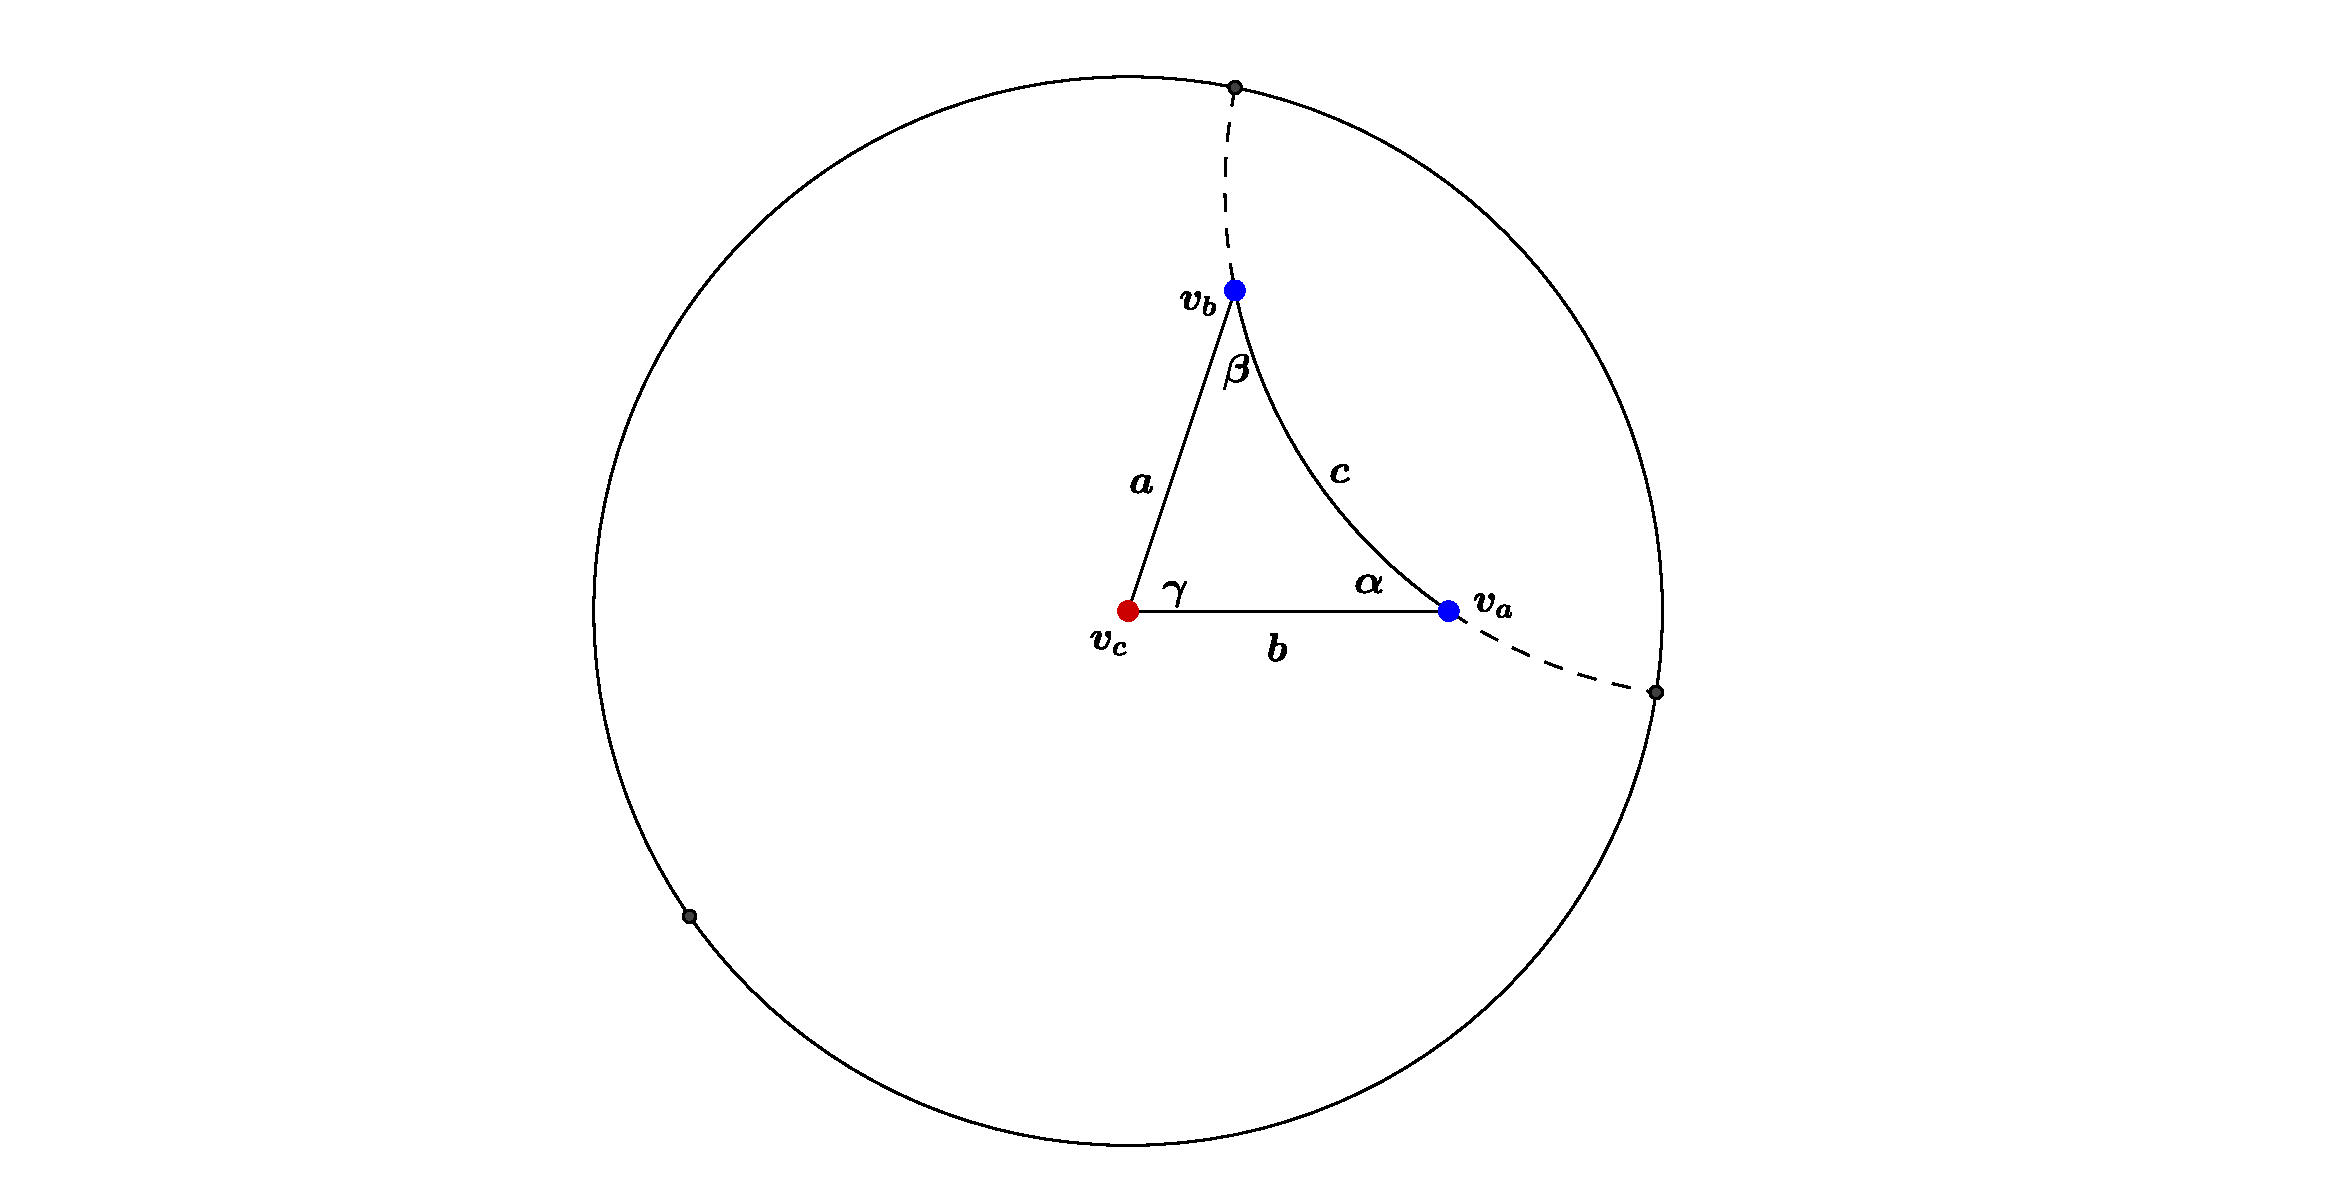
\includegraphics[width=0.8\linewidth]{images/PoincareModel.pdf}
        \caption{Đĩa Poincare $\U$}
        \label{fig:enter-label}
    \end{figure}
    Gọi các đỉnh của tam giác hyperbolic trên $\U$ lần lượt là $v_a,v_b,v_c$ với khoảng cách hyperbolic các cạnh là $a,b,c$ và các góc tương ứng $\alpha, \beta, \gamma$. Không mất tổng quát ta có thể giả sử $v_c \equiv 0, \im(v_a) = 0, \re(v_a) > 0$, khi đó 
        \[\tanh{\left(\dfrac{1}{2}\rho^*(v_a,v_c)\right)} = \left|\dfrac{v_a-0}{1-v_a\overline{0}}\right|\]
        tức $v_a = \tanh{(b/2)}$, và 
        \[\tanh{\left(\dfrac{1}{2}\rho^*(v_b,v_c)\right)} = \left|\dfrac{v_b-0}{1-v_b\overline{0}}\right|,\]
        tức $|v_b| = \tanh{(a/2)}$, dẫn đến $v_b = \tanh{(a/2)}e^{i\gamma}$.
        Từ đó suy ra
        \begin{align*}
            \cosh c &= \cosh(\rho^*(v_a,v_b)) \\
            &= 1+ 2 \sinh^2{\left(\dfrac{\rho^*(v_a,v_b)}{2}\right)}\\
            &= 1+ 2 \dfrac{|v_a -v_b|^2}{(1-|v_a|^2)(1-|v_b|^2)}\\
            &= 1+ 2 \dfrac{|\tanh{(b/2)} -\tanh{(a/2)}e^{i\gamma}|^2}{(1-\tanh^2{(b/2)})(1-\tanh^2{(a/2)})}\\
            &= 1+ 2\dfrac{|x-y(\cos{\gamma} + i \sin{\gamma})|^2}{(1-x^2)(1-y^2)} (\text{ với } x = \tanh{(b/2)}, y = \tanh{(a/2)})\\
            % &= \dfrac{(1-x^2)(1-y^2) + 2[(x-y\cos{\gamma})^2+y^2\sin^2\gamma]}{(1-x^2)(1-y^2)}\\
            &= \dfrac{x^2y^2+x^2+y^2+1}{(1-x^2)(1-y^2)}-\dfrac{4xy}{(1-x^2)(1-y^2)}\cos{\gamma}
        \end{align*}
        Mà $1-y^2 = 1 - \tanh^2{(a/2)} 
        % = 1 - \dfrac{\sinh^2(a/2)}{\cosh^2(a/2)}= \dfrac{\cosh^2(a/2)-\sinh^2(a/2)}{\cosh^2(a/2)} 
        = \dfrac{1}{\cosh^2(a/2)}$, tương tự thì 
        $1-x^2 = \dfrac{1}{\cosh^2(b/2)}$, dẫn đến 
        \begin{align*}
            &\dfrac{x^2y^2+x^2+y^2+1}{(1-x^2)(1-y^2)}\\
            &= (\tanh^2(a/2)\tanh^2(b/2) + \tanh^2(a/2) + \tanh^2(b/2) +1)\cosh^2(a/2)\cosh^2(b/2)\\
            &= \cosh^2(a/2)\cosh^2(b/2) + \sinh^2(a/2)\sinh^2(b/2) + \sinh^2(a/2)\cosh^2(b/2) + \sinh^2(b/2)\cosh^2(a/2)\\
            &= [\cosh(a/2)\cosh(b/2)+\sinh(a/2)\sinh(b/2)]^2+[\sinh(a/2)\cosh(b/2)-\sinh(b/2)\cosh(a/2)]^2\\
            &= \cosh^2\dfrac{a+b}{2} + \sinh^2\dfrac{a-b}{2}
            = \dfrac{[\cosh(a+b)+1]+[\cosh(a-b) -1]}{2}
            = \cosh a\cosh b,
        \end{align*}
        và 
        \begin{align*}
            \dfrac{4xy}{(1-x^2)(1-y^2)}
            &= 4\tanh(1/2)\tanh(b/2)\cosh^2(a/2)\cosh^2(b/2)
            % &= 4\sinh(a/2)\cosh(a/2)\sinh(b/2)\cosh(b/2)\\
            = \sinh a\sinh b.
        \end{align*}
        Vì vậy ta thu được $\cosh c = \cosh a \cosh b - \sinh a \sinh b \cos{\gamma}$.
        
        Tiếp theo ta chứng minh quy tắc $\sin$: 
        \[\dfrac{\sinh a}{\sin \alpha} = \dfrac{\sinh b}{\sin \beta} = \dfrac{\sinh c}{\sin \gamma}.\]
        Ta có 
        \begin{align*}
            \left(\dfrac{\sin{\gamma}}{\sinh c}\right)^2 
            &= \dfrac{1-\cos^2\gamma}{\sinh^2(c)}\\
            &= \dfrac{1-\left(\dfrac{\cosh a\cosh b-\cosh c}{\sinh a\sinh b}\right)^2}{\sinh^2(c)}\\
            % &= \dfrac{(\sinh a\sinh b-\cosh a\cosh b+\cosh c)(\sinh a\sinh b+\cosh a\cosh b-\cosh c)}{\sinh^2 a \sinh^2 b\sinh^2 c}\\
            % &= \dfrac{(\sinh a\sinh b-\cosh a\cosh b+\cosh c)(\sinh a\sinh b+\cosh a\cosh b-\cosh c)}{\sinh^2 a \sinh^2 b\sinh^2 c}\\
            &= \dfrac{(\cosh c-\cosh(a-b))(\cosh(a+b)-\cosh c)}{\sinh^2 a \sinh^2 b\sinh^2 c}\\
            &= \dfrac{4\sinh\dfrac{b+c-a}{2}\sinh\dfrac{c+a-b}{2}\sinh\dfrac{a+b-c}{2}\sinh\dfrac{a+b+c}{2}}{\sinh^2 a \sinh^2 b\sinh^2 c}.\\
        \end{align*}
        là một biểu thức đối xứng của $a,b,c$, tương tự cho $\dfrac{\sin \alpha}{\sinh a} \text{ và } \dfrac{\sin \beta}{\sinh b}$ ta thu được điều cần chứng minh.

        Cuối cùng ta chứng minh quy tắc $\cos II$: 
        \[\cosh{c} =\dfrac{\cos \alpha \cos \beta + \cos \gamma }{\sin \alpha \sin \beta}.\]
        Đặt $A = \cosh a, B = \cosh b, C = \cosh c$ thì
        \begin{align*}
            &\sinh a = \sqrt{A^2-1},\quad \sinh b = \sqrt{B^2-1},\quad \sinh c = \sqrt{C^2-1},\\
            &\cos \alpha = \dfrac{BC-A}{\sqrt{B^2-1}\sqrt{C^2-1}}, \quad
            \cos \beta = \dfrac{AC-B}{\sqrt{A^2-1}\sqrt{C^2-1}}, \quad 
            \cos \gamma = \dfrac{AB-C}{\sqrt{A^2-1}\sqrt{B^2-1}},\\
            &\sin \alpha = \sqrt{\dfrac{-A^2-B^2-C^2+2ABC+1}{(B^2-1)(C^2-1)}}, \quad
            \sin \beta = \sqrt{\dfrac{-A^2-B^2-C^2+2ABC+1}{(A^2-1)(C^2-1)}}.
        \end{align*}
        Suy ra 
        \begin{align*}
            \dfrac{\cos \alpha \cos \beta + \cos \gamma }{\sin \alpha \sin \beta}
            % &= \dfrac{\dfrac{BC-A}{\sqrt{B^2-1}\sqrt{C^2-1}}\dfrac{AC-B}{\sqrt{A^2-1}\sqrt{C^2-1}} + \dfrac{AB-C}{\sqrt{A^2-1}\sqrt{B^2-1}}}{\sqrt{\dfrac{-A^2-B^2-C^2+2ABC+1}{(B^2-1)(C^2-1)}}\sqrt{\dfrac{-A^2-B^2-C^2+2ABC+1}{(A^2-1)(C^2-1)}}}\\
            &= C = \cosh c.
        \end{align*}
        Kết thúc chứng minh.
\end{proof}
\begin{cor}[Định lý Pythagoras]
    Nếu $\gamma = \pi /2$ thì $\cosh c = \cosh a\cosh b$.
\end{cor}